\documentclass{beamer}
\usepackage{hyperref}
\usepackage{amsmath}
\usepackage{multirow}
\usepackage{wrapfig}
\usepackage{alltt}
\usepackage{float}
%\usepackage{subfig}
\usepackage{multirow}
\usepackage{tabularx}
\usepackage{caption}
\usepackage{subcaption}

\usetheme{beaver}
\setbeamertemplate{footline}[page number]
\setbeamertemplate{navigation symbols}{}

\AtBeginSection{\frame{\sectionpage}}
\AtBeginSubsection{\frame{\subsectionpage}}

\defbeamertemplate{section page}{mine}[1][]{%
  \begin{centering}
    {\usebeamerfont{section name}\usebeamercolor[fg]{section name}#1}
    \vskip1em\par
    \begin{beamercolorbox}[sep=12pt,center]{part title}
      \usebeamerfont{section title}\insertsection\par
    \end{beamercolorbox}
  \end{centering}
}

\defbeamertemplate{subsection page}{mine}[1][]{%
  \begin{centering}
    {\usebeamerfont{subsection name}\usebeamercolor[fg]{subsection name}#1}
    \vskip1em\par
    \begin{beamercolorbox}[sep=8pt,center,#1]{part title}
      \usebeamerfont{subsection title}\insertsubsection\par
    \end{beamercolorbox}
  \end{centering}
}

%template for Q&A slide
\defbeamertemplate{section page}{questions}[1][]{%
	\begin{centering}
		{\usebeamerfont{section name}\usebeamercolor[fg]{section name}#1}
		\vskip1em\par
		\begin{beamercolorbox}[sep=12pt,center]{part title}
			\usebeamerfont{section title}\insertsection\par
		\end{beamercolorbox}
	\end{centering}
}



\title{Helping Humans and Agents Avoid Undesirable Consequences with
Models of Intervention}
\author{Sachini Weerawardhana}
\institute{Dissertation Defense \\Advisor: Prof. Darrell Whitley}
\begin{document}
\maketitle

\begin{frame}{Agenda}
\begin{itemize}
\item \textcolor{blue} {\textbf{Introduction}}
\item Motivational study from cyber-security
\item Intervention models
\begin{itemize}
\item Intervention by recognizing actions that enable multiple undesirable consequences
\item Intervention as planning
\item Human-aware Intervention
\end{itemize}
\item Intervention recovery model
\begin{itemize}
\item The Interactive Human-aware Intervention
\end{itemize}
\end{itemize}

\end{frame} %2
\begin{frame}{The Intervention Problem}
	\begin{itemize}
		\item A human user (or an agent) is doing something online that may have an undesirable outcome that it can not recognize
		\item Two sub-problems:
		\begin{itemize}
		\item \textbf{Intervention Recognition}: Identify what the user is doing is ``bad''
		\item \textbf{Intervention Recovery}: Help the user decide what to do next
		\end{itemize}
		\item \textbf{Use automated planning as a framework to model and understand}:
		\begin{itemize}
		\item Human user behavior in cyber-security
		\item Problem solving in the Rush Hour puzzle
		\end{itemize}
	\end{itemize}
\end{frame} %3
\begin{frame}{Why is Intervention Important?}
	\begin{itemize}
		\item The actor is working in an unfamiliar environment
		\item Examples:
		\begin{itemize}
		\item Learning to use a new software application
		\item Use a computer having hidden security vulnerabilities
		\end{itemize}
		\item Intervention is a utility for online assistive agents
	\end{itemize}
\end{frame} %4
\begin{frame}{The Intervention Framework}

\begin{figure}[ptb]
 \centering{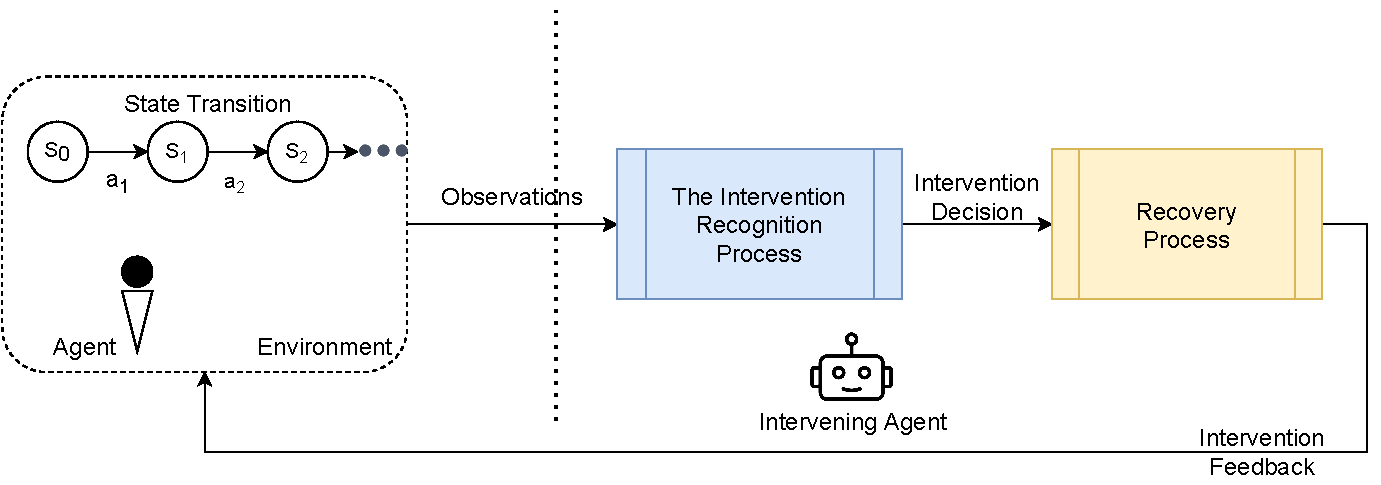
\includegraphics[width=\columnwidth]{../img/interventionrecognition.pdf}}
\end{figure}

\end{frame} %5
\begin{frame}{Thesis Outline}

\begin{figure}[tpb]
 \centering{\includegraphics[width=\columnwidth]{../img/summary.pdf}}
\end{figure}

\end{frame} %6
\begin{frame}{The Intervention Problem Dimensions}
	\begin{figure}[ptb]
 	\centering{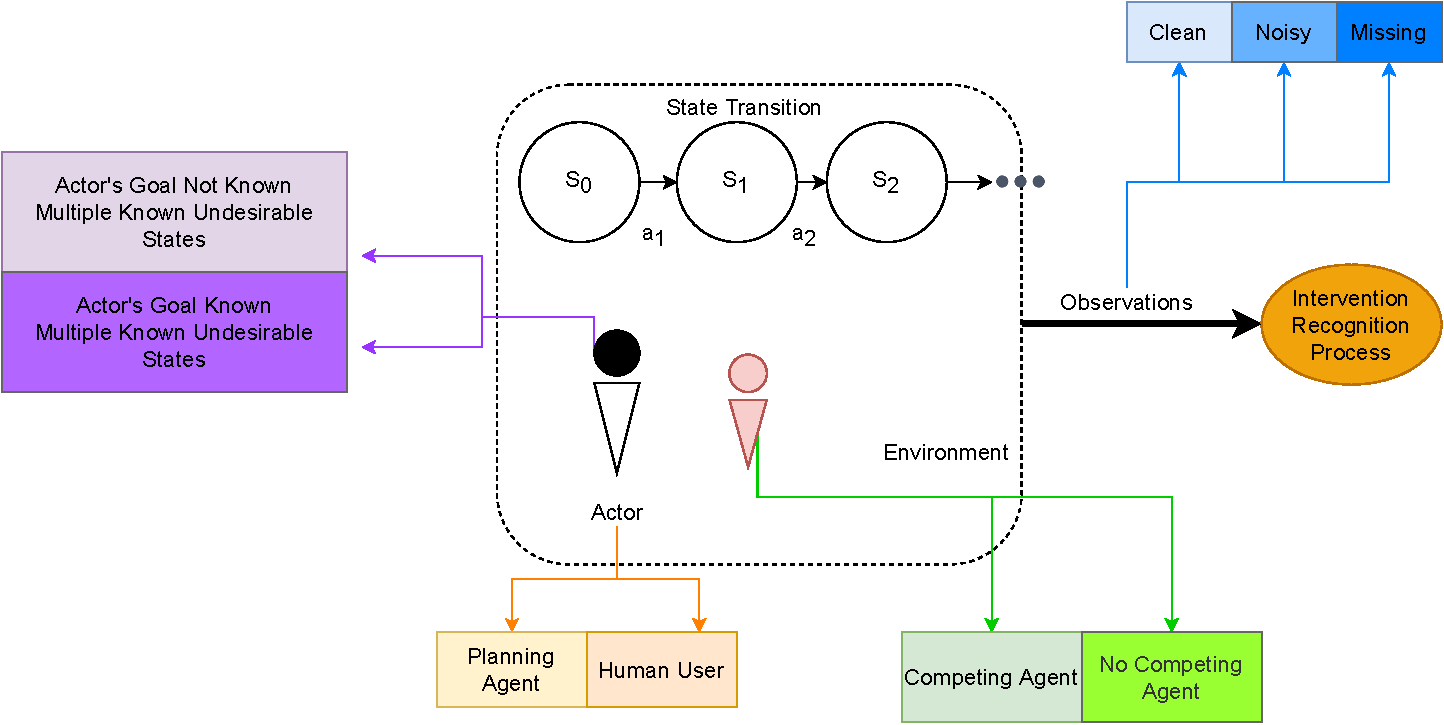
\includegraphics[width=\columnwidth]{../img/dims.pdf}}
	\end{figure}
\end{frame} %7
\begin{frame}{Undesirable States: Cyber-security Domain}

\begin{figure}[ht]
  \centering
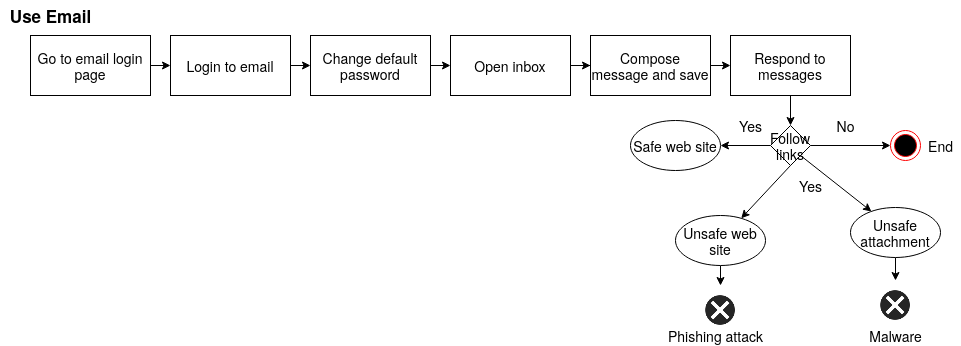
\includegraphics[width=\columnwidth, keepaspectratio=true]{img/Tasks.png}
\end{figure}

\end{frame}
  %8
\begin{frame}{Undesirable States: The Rush Hour Domain}

\begin{figure}[t]
  \centering
  \subfloat[Initial game state]{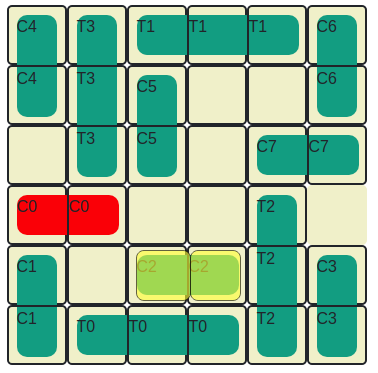
\includegraphics[width=0.4\textwidth]{img/start.png}\label{fig:start}}
  \hfill
  \subfloat[End game state]{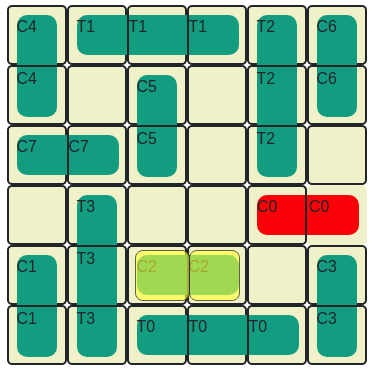
\includegraphics[width=0.4\textwidth]{img/end.png}\label{fig:end}}
  \label{fig:whole}
\end{figure}

\end{frame}
	 %9
\begin{frame}{The Gap in Existing Work}
\begin{itemize}
\item The goal/plan recognition problem 
\begin{itemize}
\item The intervening agent can infer the goal/plan of the actor using the observations as evidence
\item May not work if the actor's likely goals are too similar
\end{itemize}
\item We use machine learning to learn the differences between safe and unsafe plan suffixes.

\item The Intervention Problem:
\begin{itemize}
\item Online
\item Actors may have different views of the domain
\item Intervene on time but allow the actor to pursue his own goal
\item Intervention recovery
\end{itemize}


\end{itemize}

\end{frame} %10
\begin{frame}{Research Questions}
\begin{itemize}
\item \textbf{1: What are the salient characteristics for deciding when to intervene}?
\begin{itemize}
\item the actor's goals are known (Rush Hour)
\item the actor's goals are not known (Cyber-security)
\end{itemize}
\item \textbf{2: How to help task continuation following intervention}?
\begin{itemize}
\item Probe the search space  and inform the actor about the probes
\end{itemize}
\item \textbf{3: How to design tools to study intervention with human user participation}?
\begin{itemize}
\item Planning Domain Definition Language (PDDL) models for the two domains
\item Software tools to study human users in-situ.
\end{itemize}
\end{itemize}
\end{frame}

	 %11
\begin{frame}{Agenda}
\begin{itemize}
\item Introduction
\item \textcolor{blue} {\textbf{Motivational study from cyber-security}}
\item Intervention models
\begin{itemize}
\item Intervention by recognizing actions that enable multiple undesirable consequences
\item Intervention as planning
\item Human-aware Intervention
\end{itemize}
\item Intervention recovery model
\begin{itemize}
\item The Interactive Human-aware Intervention
\end{itemize}
\end{itemize}

\end{frame}%12
\begin{frame} {Home Computer User Behavior in Questionable Security Situations - A Motivational Study}
\begin{itemize}
\item Objectives:
\begin{itemize}
\item To capture actions taken by users when asked to perform tasks that provided ``opportunities'' to trigger security vulnerabilities
\item To assess consistency in users answers and actions.
\end{itemize}
\item Contributions:
\begin{itemize}
\item Cyber-security planning domain model for home computer security vulnerabilities
\item Software framework to support home computer user security/privacy studies
\end{itemize}
\end{itemize}
\end{frame} %13
\begin{frame}{Key Findings}
\begin{itemize}
\item Usage patterns
\begin{itemize}
\item 9+ years of experience (66\%)
\item Owned multiple devices (82\%)
\item 67\% found it challenging to identify harmful actions and take safety steps
\end{itemize}

\item Using software
\begin{itemize}
\item Users incorrectly assess self-efficacy for antivirus software installation
\item Users correctly assess self-efficacy for choosing legitimate software
\end{itemize}

\item Twitter/Email safety
\begin{itemize}
\item Users incorrectly assess self-efficacy for recognizing phishing attempts on Twitter/email
\item Users incorrectly assess self-efficacy for identifying malicious attachments
\end{itemize}
\end{itemize}
\end{frame}

\begin{frame}{Key Findings}
\begin{itemize}
\item Recognizing system cues for safety
\begin{itemize}
\item Web page content helps users select safe software to download
\item HTTPS/padlock icon helps users recognize safe web pages to download software
\item HTTPS/padlock icon does not help users recognize phishing links on Twitter
\item HTTPS/padlock icon does not help users recognize phishing links while using email
\end{itemize}
\end{itemize}

\end{frame} %14, 15
\begin{frame} {Designing Intervention for Cyber-security Domain}
\begin{itemize}
\item Home computer users might not think about the post-conditions of actions while performing common tasks
\item Home computer users might not perceive preconditions that exist in the state (e.g., padlock icons/HTTPS)

\item Intervention solution needs to address:
\begin{itemize}
\item Users do not complete tasks methodically (e.g., repeated actions, skips) $\Rightarrow$ \texttt{noise in observations}
\item Intervention must be decided as and when observations become available  $\Rightarrow$ \texttt{online operation}
\item Need to evaluate proximity to an exploit regardless of the user's goal $\Rightarrow$ \texttt{user's desirable goal is unknown}
\end{itemize}
\end{itemize}
\end{frame} %16
\begin{frame}{Agenda}
\begin{itemize}
\item Introduction
\item Motivational study from cyber-security
\item \textcolor{blue} {\textbf{Intervention models}}
\begin{itemize}
\item \textcolor{blue} {\textbf{Intervention by recognizing actions that enable multiple undesirable consequences}}
\item Intervention as planning
\item Human-aware Intervention
\end{itemize}
\item Intervention recovery model
\begin{itemize}
\item The Interactive Human-aware Intervention
\end{itemize}
\end{itemize}

\end{frame} %17
\begin{frame} {Intervention by Recognizing Actions That Enable Multiple Undesirable Consequences}
\begin{itemize}

\item Need to identify an action that causes the most damage and least interferes with the user's needs
\item Contribution:
\begin{itemize}
\item Undesirable Consequences Recognition Function
\item Domain-independent metrics to measure the importance of an observed action towards contributing to multiple undesirable states
\end{itemize}

\end{itemize}

\end{frame} %18
\begin{frame} {Intervention Problem Dimensions}

	\begin{figure}[ptb]							\centering{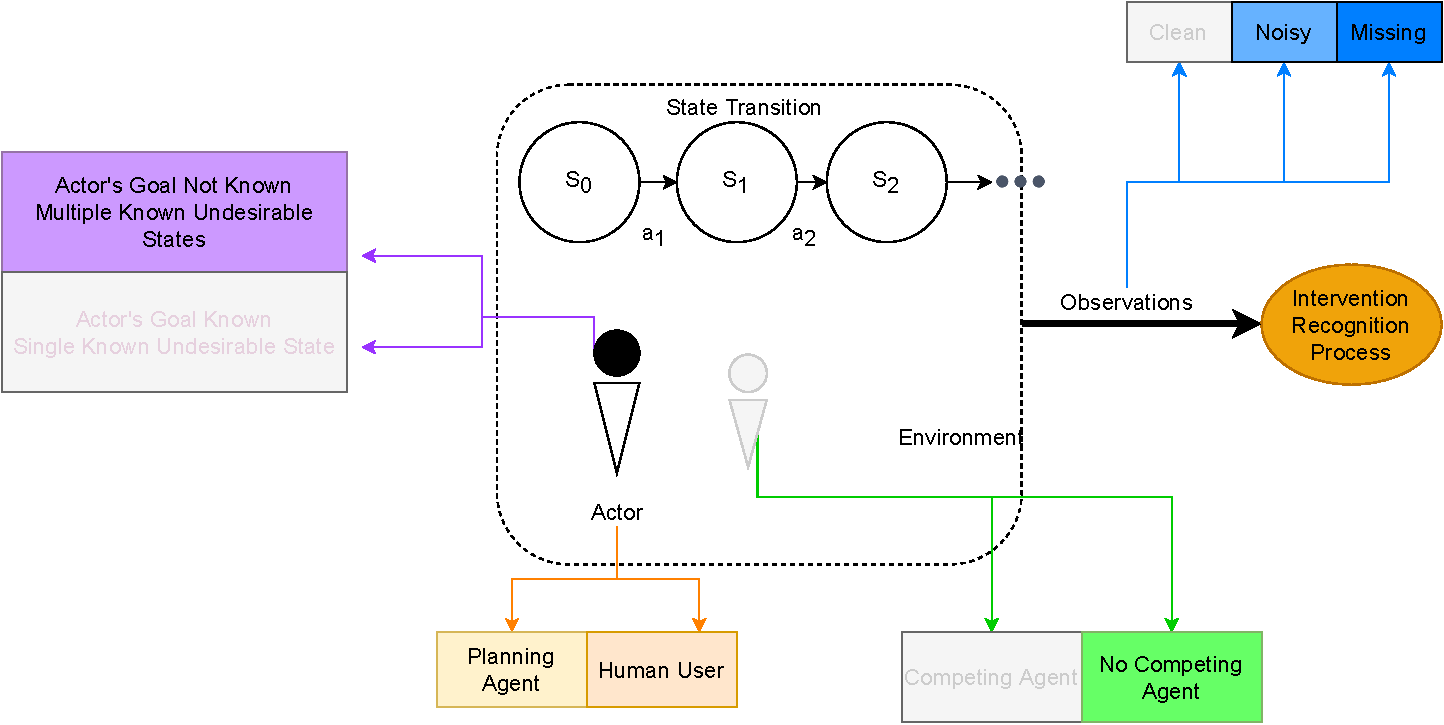
\includegraphics[width=\columnwidth]{../img/ch4.pdf}}
	\end{figure}
	
\end{frame} %19
%\begin{frame}{Salient Characteristics for Deciding to Intervene}
%\begin{itemize}
%\item Model the environment as a STRIPS style planning domain
%\item Use an automated planner to sample plans for the undesirable states
%\end{itemize}
%	\begin{figure}[t]
%		\centering{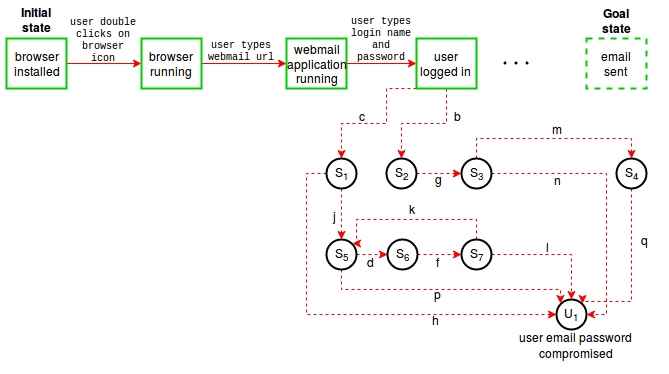
\includegraphics[width=0.7\columnwidth]{states.png}}
%	\end{figure}
%Observation trace\\ $[$\texttt{{\small user double clicks on browser icon, user types webmail url, user types login name and password}}$]$
%
%\end{frame}


\begin{frame}{Salient Characteristics for Deciding to Intervene}
	\begin{itemize}
		\item Certainty (C)
		\begin{itemize}
			\item How many plans contained the action over the number of sampled plans
			\item Highlight frequently occurring actions in plans as important
		\end{itemize}
		
		\item Timeliness (T)
			\begin{itemize}
				\item Maximum normalized steps remaining in the sampled plans
				\item Quantifies how soon the undesirable state may occur
			\end{itemize}
		
		\item Desirability (D)	
		\begin{itemize}
			\item Number of times the action appears in the sampled plans over the sum of actions in the sampled plans
			\item Separate common harmless actions that further the user’s actual goal from harmful actions to be avoided
			\item Negative metric
		\end{itemize}
		
	\end{itemize}
\end{frame}


\begin{frame}{Undesirable Consequences Recognition Function}
	\begin{itemize}
	\item Critical Trigger Action is an observed action that maximizes $V(a)$:
	
		\begin{align*}
		V(a) &= \alpha_1 * Certainty (a|\Pi_U) +\;\alpha_2 * Timeliness (a|\Pi_U) \\ &-\;\alpha_3 * Desirability (a|\Pi_U)
		\end{align*}
		
		\item $a  $ candidate action from the sampled undesirable plans plans
		\item $\Pi_U  $ sampled undesirable plans
		\item $(\alpha_1, \alpha_2, \alpha_3)  $ metric weight assignments
	\end{itemize}

\end{frame} %20, 21
\begin{frame}{Experiments}
	\begin{itemize}
		\item Planning domain from the home computer cyber-security study
		\item Four benchmark planning domains (Blocks words, navigator, ipc-grid+, logistics)

		\item Four undesirable states for each domain
		\item Observation traces of actions
		\begin{itemize}
			\item Activity logs (n=61) captured during the human subject study
			\item Synthetic traces generated with controlled levels of noise and missing actions for benchmark domains
		\end{itemize}
		\item Metric weights
		\begin{itemize}
			\item 7 classes of discrete weight assignments for the three metrics
			\item (1,0,0), (0,1,0), (0,0,1), (.33,.33,.33), (.5,.5,0), (.5,0,.5), (0,.5,.5)
		\end{itemize}
	\end{itemize}
\end{frame} %22
\begin{frame}{Key Findings - Cyber-security Domain}

\begin{itemize}
\item For each decision cycle, the selected critical trigger action is correct if it is in a ground truth undesirable plan

\begin{itemize}
\item Mean accuracy = 59.53\% (SD=30.79) across the 7 metric weight assignment classes
\end{itemize}

\item Effect of metric weights on accuracy is significant ($F=40866, p<<0$)
\item Highest accuracy (mean=95.59\%,SD=2.13) for two classes
\begin{itemize}
\item Equal weights for C, T, D
\item Equal weights for C, T ignoring D
\end{itemize}

\item Dominant metrics: \textbf{Certainty} and \textbf{Timeliness}
\end{itemize}

\end{frame}

\begin{frame}{Key Findings - Benchmark Synthetic Domains}

\begin{itemize}
\item Percentage of extraneous actions not flagged as critical

\begin{figure}
     \centering
     \begin{subfigure}[b]{0.5\columnwidth}
         \centering
                  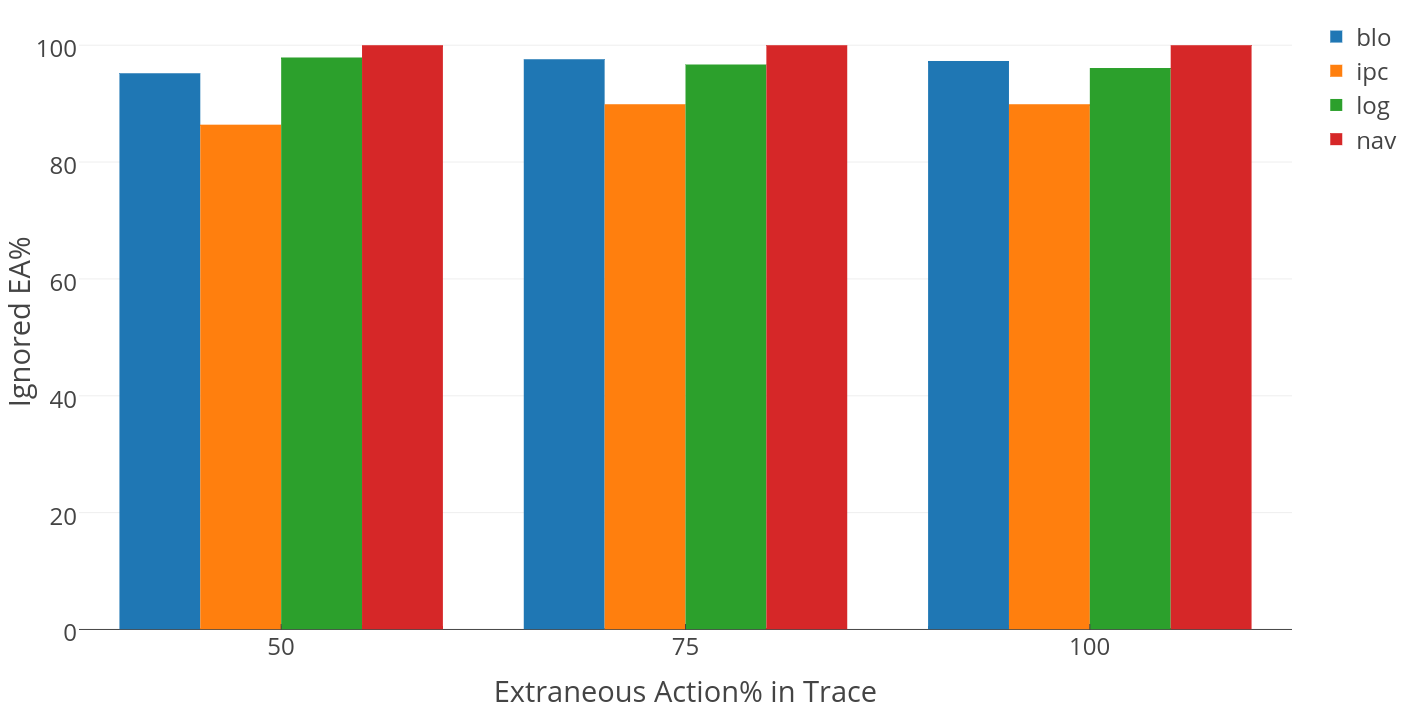
\includegraphics[width=\textwidth]{../img/ignoredea.png}
     \end{subfigure}
     \begin{subfigure}[b]{0.5\columnwidth}
         \centering
                  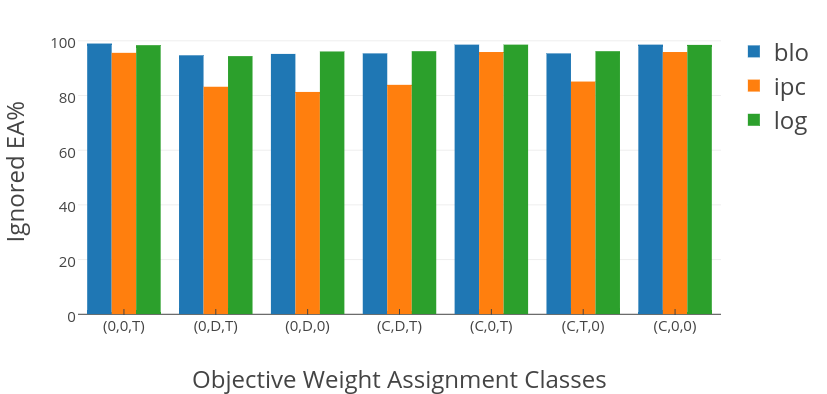
\includegraphics[width=\textwidth]{../img/ow.png}
     \end{subfigure}
\end{figure}

\item Metric weights significantly influence ignoring extraneous actions
\begin{itemize}
\item Dominant metrics: \textbf{Certainty}, \textbf{Desirability}
\end{itemize}
\end{itemize}

\end{frame}


\begin{frame}
\begin{itemize}
\item Percentage of ground truth undesirable actions flagged as critical
\item  Low rates indicate that other factors in addition to the three metrics may influence flagging  undesirable actions
\item Metric weights significantly influence flagging undesirable actions
\begin{itemize}
\item Dominant metrics: \textbf{Timeliness}
\end{itemize}
\end{itemize}
\begin{figure}
     \centering
      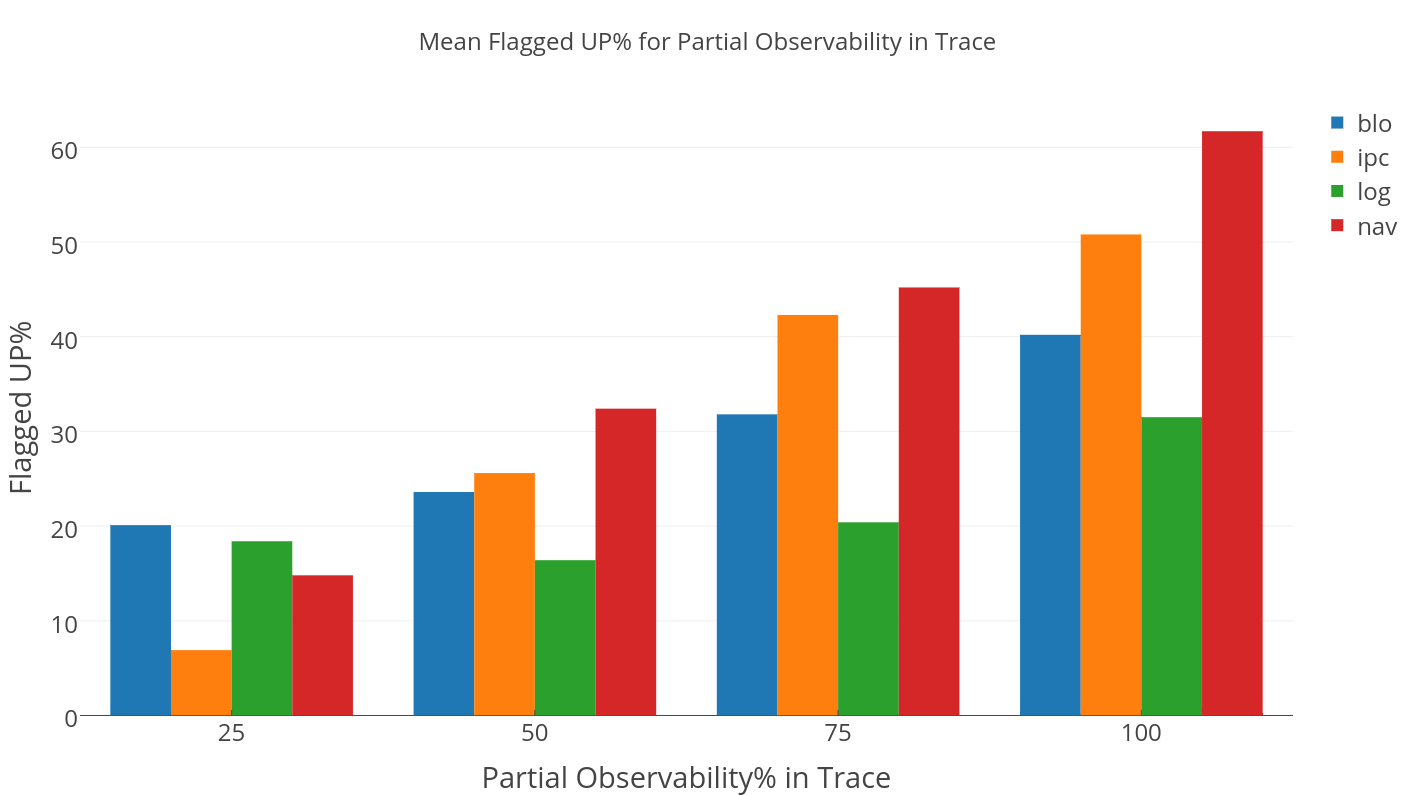
\includegraphics[width=0.7\textwidth]{../img/flaggedup.png}
\end{figure}

\end{frame}

%\begin{frame}{Summary}
%\begin{itemize}
%\item Model the domain as a planning problem 
%\item Use automated planning to sample the intervening agent's decision space
%\item Undesirable Consequences Recognition Function to rank candidate critical actions
%\item Metric weighting affects the ability to ignore extraneous actions and correctly flag true positives with partial observability
%\end{itemize}
%\end{frame} %23, 24, 25
\begin{frame}{Agenda}
\begin{itemize}
\item Introduction
\item Motivational study from cyber-security
\item \textcolor{blue} {\textbf{Intervention models}}
\begin{itemize}
\item Intervention by recognizing actions that enable multiple undesirable consequences
\item \textcolor{blue} {\textbf{Intervention as planning}}
\item Human-aware Intervention
\end{itemize}
\item Intervention recovery model
\begin{itemize}
\item The Interactive Human-aware Intervention
\end{itemize}
\end{itemize}

\end{frame}%26
\begin{frame}{Intervention as Planning}
\begin{itemize}
\item Combines machine learning and automated planning
\item Solution is based on plan suffix analysis
\item Identify different characteristics between solutions obtained from an automated planner that contain undesirable actions and solutions that do not
\item Hidden effects in the environment
\begin{itemize}
\item a competitor using a hidden object to subvert the actor's goal
\item a pothole the actor can not see
\end{itemize}
\end{itemize}
\end{frame} %27
\begin{frame} {Intervention as Planning: Problem Dimensions}

	\begin{figure}[ptb]							\centering{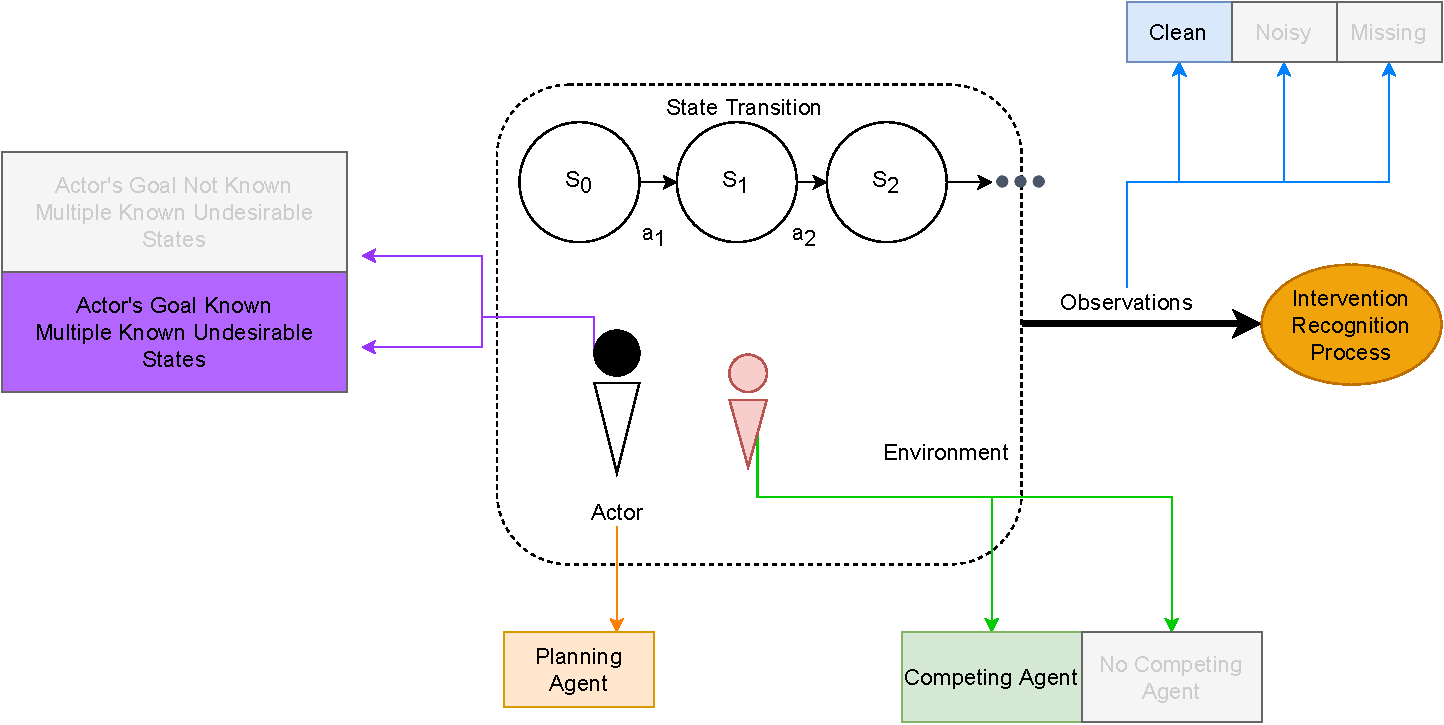
\includegraphics[width=\columnwidth]{../img/knowngoals.pdf}}
	\end{figure}
	
\end{frame} %28
\begin{frame}{Learning to Intervene}
\begin{itemize}
\item Two feature sets:
\begin{itemize}
\item Metrics from \textbf{The Intervention Graph}
\item Plan distance measures from the sampled plans
\end{itemize}
\item Use the feature sets to train classifiers to recognize actions that should be flagged for intervention
\begin{itemize}
\item Naive Bayes, K-nearest neighbor, Decision tree, Logistic regression
\end{itemize}
\end{itemize}

\end{frame}


\begin{frame}{The Intervention Graph}
\begin{itemize}
\item Produce the intervention graph from current state (root) to $G_1$ (BAD) and $G_0$ (TAD) (leaves)
\end{itemize}

\begin{figure}[tb]
        \centering{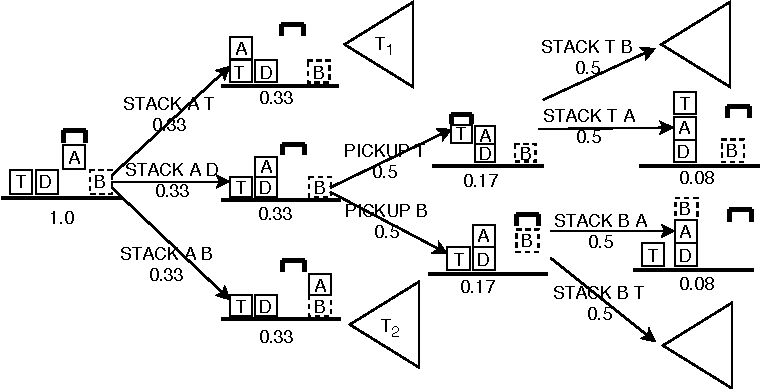
\includegraphics[width=\columnwidth]{img/featuresbw.pdf}}
\end{figure} 

\end{frame}


\begin{frame} {Intervention Graph Features}
\begin{itemize}
\item \textbf{Risk} - Posterior probability of reaching $G_1$, when the user is trying to reach $G_0$
\item \textbf{Desirability} - Posterior probability of reaching $G_0$, without passing $G_1$
\item \textbf{Distance to} $G_0$ - Mean number of edges between the root of the tree and $G_0$, which doesn't pass through $G_1$
\item \textbf{Distance to} $G_1$ - Mean number of edges between the root of the tree and $G_1$
\item \textbf{Active attack landmarks\%} - From the total number of predicates that must be true in any valid solution to the planning problem $\langle M,G_1\rangle$, how many are true in the current state?
\end{itemize}

\end{frame}

\begin{frame} {Plan Distance Measures From Sampled Plans}
\begin{itemize}
\item Instead of computing exact distances and probabilities \textbf{compute an estimated proximity} to $G_0$ and $G_1$
\item Use an automated planner to find two sets of solutions for $\langle M, G_0\rangle$ and $\langle M, G_1 \rangle$
\item Compute a \textbf{reference plan} $ = \lbrace observations + \pi_* \rbrace$
\item Compute the plan distances between the  \textbf{reference plan} and the plans in $\langle M, G_0\rangle$ and $\langle M, G_1 \rangle$
\end{itemize}

\end{frame} %29, 30, 31, 32
\begin{frame} {Classifier Performance}
Reporting $F-score = \frac{TP}{TP+1/2(FP+FN)}$\\
Matthews Correlation Coefficient (MCC)

\begin{table}[ptb]
\resizebox{\textwidth}{!}{%
\begin{tabular}{|l|ll|ll|ll|ll|ll|ll|}
\hline
\multicolumn{1}{|c|}{\multirow{3}{*}{Domain}} & \multicolumn{6}{c|}{Logistic Regression} & \multicolumn{6}{c|}{K-Nearest} \\ \cline{2-13} 
\multicolumn{1}{|c|}{} & \multicolumn{2}{c|}{Test Set 1} & \multicolumn{2}{c|}{Test Set 2} & \multicolumn{2}{c|}{Test Set 3} & \multicolumn{2}{c|}{Test Set 1} & \multicolumn{2}{c|}{Test Set 2} & \multicolumn{2}{c|}{Test Set 3} \\ \cline{2-13} 
\multicolumn{1}{|c|}{} & \multicolumn{1}{l|}{F-score} & MCC & \multicolumn{1}{l|}{F-score} & MCC & \multicolumn{1}{l|}{F-score} & MCC & \multicolumn{1}{l|}{F-score} & MCC & \multicolumn{1}{l|}{F-score} & MCC & \multicolumn{1}{l|}{F-score} & MCC \\ \hline
\multicolumn{13}{|c|}{Intervention Graph Method} \\ \hline
\textbf{Blocks-1} & 1 & 1 & 1 & 1 & 1 & 1 & 1 & 1 & 1 & 1 & 1 & 1 \\ \cline{1-1}
\textbf{Blocks-2} & 1 & 1 & 1 & 1 & 1 & 1 & 1 & 1 & 1 & 1 & 1 & 1 \\ \cline{1-1}
\textbf{EasyIPC} & .88 & .87 & .88 & .87 & .86 & .86 & 1 & 1 & 1 & 1 & 1 & 1 \\ \cline{1-1}
\textbf{Ferry} & 1 & 1 & 1 & 1 & 1 & 1 & 1 & 1 & 1 & 1 & 1 & 1 \\ \cline{1-1}
\textbf{Navigator} & 1 & 1 & 1 & 1 & .99 & .99 & 1 & 1 & .96 & .96 & .99 & .99 \\ \hline

\multicolumn{13}{|c|}{Plan Space Sampling Method} \\ \hline
\textbf{Blocks-1} & .25 & .33 & .25 & .33 & .25 & .33 & 1 & 1 & 1 & 1 & 1 & 1 \\ \cline{1-1}
\textbf{Blocks-2} & 1 & 1 & 1 & 1 & 1 & 1 & 1 & 1 & 1 & 1 & 1 & 1 \\ \cline{1-1}
\textbf{EasyIPC} & .64 & .63 & .46 & .44 & .67 & .66 & .05 & -.04 & .04 & -.03 & .05 & -.02 \\ \cline{1-1}
\textbf{Ferry} & .31 & .32 & .23 & .22 & 1 & 1 & .33 & .40 & .13 & .15 & .81 & .82 \\ \cline{1-1}
\textbf{Navigator} & .60 & .59 & .98 & .94 & .97 & .97 & .61 & .65 & 1 & 1 & 1 & 1 \\ \hline
\end{tabular}%
}
\end{table}

\end{frame}

\begin{frame} {Intervention Using Existing Goal Recognition Algorithms}
RG (LAMA) - Probabilistic goal recognition using a satisificing planner\\


\begin{table}[ptb]
\begin{tabular}{|l|ll|ll|ll|}
\hline
\multicolumn{1}{|c|}{\multirow{2}{*}{Domain}} & \multicolumn{2}{c|}{Test Set 1} & \multicolumn{2}{c|}{Test Set 2} & \multicolumn{2}{c|}{Test Set 3} \\ \cline{2-7} 
\multicolumn{1}{|c|}{} & \multicolumn{1}{c|}{F-score} & \multicolumn{1}{c|}{MCC} & \multicolumn{1}{c|}{F-score} & \multicolumn{1}{c|}{MCC} & \multicolumn{1}{c|}{F-score} & \multicolumn{1}{c|}{Mcc} \\ \hline
\textbf{Blocks-1} & .38 & .45 & .43 & .49 & .40 & .47 \\ \cline{1-1}
\textbf{Blocks-2} & 1 & 1 & .9 & .9 & 1 & 1 \\ \cline{1-1}
\textbf{EasyIPC} & .13 & .05 & .21 & .17 & .23 & .19 \\ \cline{1-1}
\textbf{Ferry} & .17 & .18 & .22 & .23 & .15 & .17 \\ \hline
\end{tabular}
\end{table}
\end{frame} %33, 34
\begin{frame}{Agenda}
\begin{itemize}
\item Introduction
\item Motivational study from cyber-security
\item \textcolor{blue} {\textbf{Intervention models}}
\begin{itemize}
\item Intervention by recognizing actions that enable multiple undesirable consequences
\item Intervention as planning
\item \textcolor{blue} {\textbf{Human-aware Intervention}}
\end{itemize}
\item Intervention recovery model
\begin{itemize}
\item The Interactive Human-aware Intervention
\end{itemize}
\end{itemize}

\end{frame}%35
\begin{frame}{Human-aware Intervention}
\begin{itemize}
\item The actor is a human user. We cannot approximate plan suffixes using automated planners
\item Observe how human users solve Rush Hour puzzles
\item What did the users who did not move the forbidden vehicle do
differently than those who moved the forbidden vehicle?
\end{itemize}

\end{frame} %36
\begin{frame}{Human-aware Intervention - Problem Dimensions}
	\begin{figure}[ptb]							\centering{\includegraphics[width=\columnwidth]{../img/human-aware.pdf}}
	\end{figure}
\end{frame} %37
\begin{frame}{Human-aware Intervention - Behavior Study}
\begin{itemize}
\item In Web-based puzzle simulator app, subjects solve one
randomly assigned Rush Hour puzzle.
\item Subjects are told the puzzle has one forbidden vehicle that
need not be moved
\item No alerts if the forbidden vehicle is moved
\item Post-study survey of demographics and puzzle solving habits
\item 136 university students from different
departments
\end{itemize}

\end{frame} %38
\begin{frame}{Key Findings}
\begin{itemize}
\item Huge enthusiasm for puzzle solving tasks (78\%)
\item 49\% moved the forbidden vehicle
\item Behavior patterns in unsafe solutions
\begin{itemize}
\item Moving the same car back and forth in succession (do/undo)
\item Making moves that clears space around the forbidden vehicle
\item Lengthy solution : \textbf{statistically significant positive correlation} between the solution length and the number of times the forbidden vehicle was moved
\end{itemize}

\end{itemize}

\end{frame}

%\begin{frame} {Key Findings}
%\begin{table}[ptb]
%\begin{tabular}{|l|l|l|l|l|l|l|}
%\hline
%\multicolumn{1}{|c|}{\multirow{2}{*}{PID}} &
%  \multicolumn{2}{c|}{Fast (46)} &
%  \multicolumn{2}{c|}{Medium (42)} &
%  \multicolumn{2}{c|}{Slow (48)} \\ \cline{2-7} 
%\multicolumn{1}{|c|}{} &
%  \multicolumn{1}{c|}{Mean} &
%  \multicolumn{1}{c|}{\begin{tabular}[c]{@{}c@{}}Forbidden\\ Moves\end{tabular}} &
%  \multicolumn{1}{c|}{Mean} &
%  \multicolumn{1}{c|}{\begin{tabular}[c]{@{}c@{}}Forbidden\\ Moves\end{tabular}} &
%  \multicolumn{1}{c|}{Mean} &
%  \multicolumn{1}{c|}{\begin{tabular}[c]{@{}c@{}}Forbidden\\ Moves\end{tabular}} \\ \hline
%P1  & 25.5 & 0  & 41.7  & 0  & 64.7  & 0  \\ 
%P2  & 74.7 & 4  & 137.7 & 16 & 277   & 28 \\ 
%P3  & 26.5 & 8  & 36.2  & 9  & 43.7  & 6  \\ 
%P4  & 25.2 & 1  & 32    & 4  & 76    & 28 \\ 
%P5  & 18.3 & 3  & 26    & 2  & 44.75 & 13 \\ 
%P6  & 22   & 0  & 24.5  & 0  & 39.6  & 0  \\ 
%P7  & 38.5 & 5  & 53.3  & 16 & 120   & 37 \\ 
%P8  & 9    & 0  & 9     & 0  & 10    & 0  \\ 
%P9  & 27.8 & 8  & 48.6  & 12 & 99    & 28 \\ 
%P10 & 50.3 & 11 & 66    & 14 & 127.3 & 46 \\ \hline
%\end{tabular}
%\caption{Plans produced by human users grouped by the mean number of moves and the number of forbidden moves}
%\label{tab:solvergroups}
%\end{table}
%\end{frame} %39
\begin{frame}{Learning Human-aware Intervention}
\begin{itemize}
\item Game state based features
\begin{itemize}
\item number of times a move increased the number of cars blocking the goal car’s path
\item number of times a move freed up empty spaces around the forbidden vehicle
\item number of times the number of empty spaces around the forbidden vehicle blockers increased
\item mean number of empty spaces around the goal and forbidden car blockers
\end{itemize}
\item User action based features
\begin{itemize}
\item number of moves in the user's solution
\item difference of number of moves to the cost optimal solution
\item number of vehicles moved
\item number of times a move was immediately undone
\end{itemize}
\end{itemize}
\end{frame} %40
\begin{frame}{Classifier Performance}
\begin{itemize}
\item Intervention accuracy while offering three levels of freedom $k=\lbrace 1,2,3\rbrace$
\item 70-30 split for training and test sets
\item Classifiers trained with 10-fold cross validation
\end{itemize}

\begin{table}[tpb]

\resizebox{\textwidth}{!}{%
\begin{tabular}{|l|l|l|l|l|l|l|l|l|l|}
\hline
\multicolumn{1}{|c|}{\multirow{2}{*}{Classifier}} & \multicolumn{3}{c|}{$k=1$} & \multicolumn{3}{c|}{$k=2$} & \multicolumn{3}{c|}{$k=3$} \\ \cline{2-10} 
\multicolumn{1}{|c|}{} & \multicolumn{1}{c|}{Precision} & Recall & F-score & Precision & Recall & F-score & Precision & Recall & F-score \\ \hline
Decision Tree & 0.70 & 0.90 & 0.89 & 0.80 & 0.95 & 0.87 & 0.89 & 0.81 & 0.85 \\ \cline{1-1}
KNN & 0.89 & 0.76 & 0.82 & 0.86 & 0.86 & 0.86 & \textbf{0.95} & \textbf{0.90} & \textbf{0.93} \\ \cline{1-1}
Logistic Regression & \textbf{0.91} & \textbf{0.95} & \textbf{0.93} & \textbf{0.87} & \textbf{1} & \textbf{0.93} & \textbf{0.91} & \textbf{0.95} & \textbf{0.93} \\ \cline{1-1}
Naive Bayes & 0.73 & 0.90 & 0.81 & 0.74 & 0.86 & 0.83 & 0.68 & 0.90 & 0.78 \\ \hline
\end{tabular}
}%
\end{table}

\begin{itemize}
\item Predict intervention using the Probabilistic Plan Recognition Algorithm  (Ramirez and Geffener, 2010)
\end{itemize}

\begin{table}[tpb]
\resizebox{\textwidth}{!}{%
\begin{tabular}{|l|l|l|l|l|l|l|l|l|l|}
\hline
\multirow{2}{*}{Goal Priors} & \multicolumn{3}{c|}{$k=1$} & \multicolumn{3}{c|}{$k=2$} & \multicolumn{3}{c|}{$k=3$} \\ \cline{2-10} 
 & Precision & Recall & F-score & Precision & Recall & F-score & Precision & Recall & F-score \\ \hline
Uniform & 0.67 & 0.56 & 0.61 & 0.67 & 0.56 & 0.61 & 0.56 & 0.67 & 0.61 \\ \cline{1-1}
$P$($\mathrm{u}$) = 2$\times P$($\mathrm{d}$) & 0.69 & 0.61 & 0.65 & 0.69 & 0.61 & 0.65 & 0.69 & 0.61 & 0.65 \\ \cline{1-1}
$P$($\mathrm{d}$) = 2$\times P$($\mathrm{u}$) & 0.67 & 0.56 & 0.61 & 0.67 & 0.56 & 0.61 & 0.67 & 0.56 & 0.67 \\ \hline
\end{tabular}
}%
\label{tab:prp}
\end{table}

\end{frame} %41
\begin{frame}{Summary}
\begin{itemize}
\item Introduced a family of Intervention Problems
\begin{itemize}
\item Intervention for a single actor (planning agent)
\item Intervention for an actor in the presence of a competitor (planning agents)
\item Human-Aware Intervention for a single actor (human user)
\end{itemize}
\item Solutions
\begin{itemize}
\item If the actor is a planning agent - Plan Suffix Analysis
\item If the actor is a human user -  Observed History Analysis
\end{itemize}
\item Proposed learning based intervention outperforms existing plan recognition algorithms
\end{itemize}
\end{frame} %42
\begin{frame}{Agenda}
\begin{itemize}
\item Introduction
\item Motivational study from cyber-security
\item Intervention models
\begin{itemize}
\item Intervention by recognizing actions that enable multiple undesirable consequences
\item Intervention as planning
\item Human-aware Intervention
\end{itemize}
\item \textcolor{blue} {\textbf{Intervention recovery model}}
\begin{itemize}
\item \textcolor{blue} {\textbf{The Interactive Human-aware Intervention}}
\end{itemize}
\end{itemize}

\end{frame} %43
\begin{frame}{Interactive Human-aware Intervention}
\begin{itemize}
\item Study intervention recovery in a Rush Hour planning task
\item The intervening agent helps the user modify the current trajectory of the plan by providing the hints about the search space of the planning problem.
\item Hints:
\begin{itemize}
\item The minimum remaining number of moves
\item The next best move
\item The vehicles that must be moved
\item Restart puzzle
\end{itemize}
\end{itemize}
\end{frame} %44
\begin{frame}{Gap in Existing Work}
\begin{itemize}
\item Improving human-agent collaborations with explanations
\item When the intervening agent (has knowledge advantage) does something the human user does not expect, Explainable AI has been used to enable transparency.
\item Explain the surprise using different modalities
\begin{itemize}
\item plan visualization techniques to help human users understand the solution produced by an automated planner
\item question answer dialog (``why did you do A?'', ``why not B?'')
\end{itemize}
\item Hints are designed to help the user uncover information about the Rush Hour planning problem
\end{itemize}
\end{frame} %45
\begin{frame}{Interactive Human-aware Intervention - Behavior Study}
\begin{itemize}
\item In Web-based puzzle simulator app, human subjects solve one randomly assigned Rush Hour puzzle assisted by the Human-aware Intervention agent
\item Participants were randomly assigned to also watch a help video to learn how to avoid the forbidden vehicle
\item Subjects are told the puzzle has one forbidden vehicle and the puzzle can be solved without it
\item When forbidden vehicle is moved subjects see an alert message
\item Post-study survey of demographics and hint helpfulness rating
\item 135 university students from different departments
\end{itemize}
\end{frame} %46
\begin{frame}{Key Findings}
\begin{itemize}
\item Statistically significant positive correlation between the solution length and the number of times the forbidden vehicle was moved
\item Most requested hint : \textbf{Show the Next Best Move}
\begin{itemize}
\item Slow/medium/fast solvers
\item Three puzzle classes C, E, M
\end{itemize}
\end{itemize}
\end{frame}
 %47
\begin{frame}{Hint Request Distribution}

\begin{figure}[tpb]
  \centering
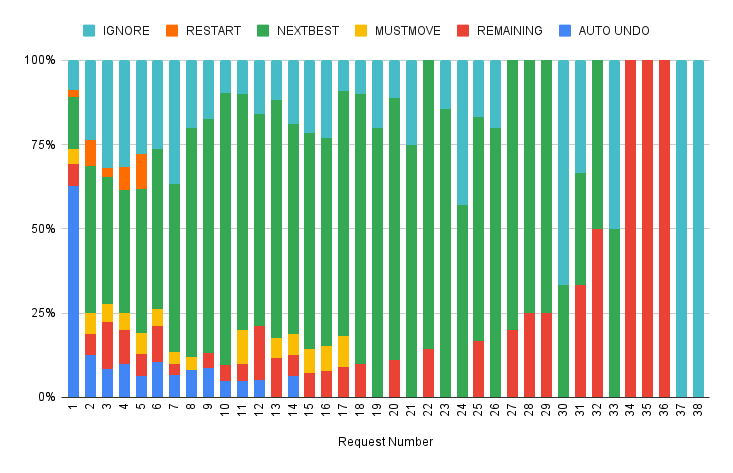
\includegraphics[width=0.9\columnwidth]{../img/reqdistribution.png}
  \caption{Percentage split for hints for each request number}
  \label{fig:reqdistribution}
\end{figure}

\end{frame} %48
\begin{frame}{Qualitative Evaluation}
\begin{table}[tbp]
\caption{\textbf{H1}: Show the minimum remaining number of moves, \textbf{H2}: Show the next best move, \textbf{H3}: Show the vehicles that must be moved, \textbf{H4}: restart puzzle}
\resizebox{\textwidth}{!}{%
\begin{tabular}{lll|l|l|l|l|}
\cline{4-7}
 &  &  & \multicolumn{4}{l|}{\textbf{Mean (std. dev.) helpfulness rating}} \\ \hline
\multicolumn{1}{|l|}{\textbf{Type}} & \multicolumn{1}{l|}{\textbf{Puzzle ID}} & \textbf{Count} & \multicolumn{1}{c|}{H1} & \multicolumn{1}{c|}{H2} & \multicolumn{1}{c|}{H3} & \multicolumn{1}{c|}{H4} \\ \hline
\multicolumn{1}{|l|}{\multirow{4}{*}{\textbf{C}}} & \multicolumn{1}{l|}{P2} & 6 & 1.5 (2.5) & \textbf{4.3} (2.6) & 3.8 (2.3) & 2.0 (2.3) \\
\multicolumn{1}{|c|}{} & \multicolumn{1}{l|}{P4} & 11 & 1.3 (2.1) & \textbf{2.3} (2.1) & 1.5 (2.2) & 0.8 (1.7) \\
\multicolumn{1}{|c|}{} & \multicolumn{1}{l|}{P6} & 3 & 2.0 (1.2) & \textbf{3.3} (2.6) & 1.7 (2.9) & 0 \\
\multicolumn{1}{|c|}{} & \multicolumn{1}{l|}{P8} & 1 & 0 & \textbf{3.0} & \textbf{3.0} & 1.0 \\ \hline
\multicolumn{1}{|l|}{\multirow{5}{*}{\textbf{E}}} & \multicolumn{1}{l|}{P1} & 4 & 1.5 (1.3) & \textbf{4.3} (1.0) & 3.8 (1.9) & 2.0 (2.2) \\
\multicolumn{1}{|l|}{} & \multicolumn{1}{l|}{P3} & 13 & 1.3 (1.6) & \textbf{2.3} (2.2) & 1.5 (1.7) & 0.8 (0.9) \\
\multicolumn{1}{|l|}{} & \multicolumn{1}{l|}{P5} & 13 & 1.4 (1.3) & \textbf{2.2} (1.9) & \textbf{2.2} (2.0) & 1.8 (1.9) \\
\multicolumn{1}{|l|}{} & \multicolumn{1}{l|}{P9} & 7 & 0.9 (1.2) & \textbf{1.7} (2.2) & 1.1 (1.7) & 1.3 (2.0) \\
\multicolumn{1}{|l|}{} & \multicolumn{1}{l|}{P10} & 8 & 0.9 (1.0) & \textbf{2.8} (2.3) & 1.6 (1.5) & \textbf{2.8} (2.1) \\ \hline
\multicolumn{1}{|l|}{\multirow{4}{*}{\textbf{M}}} & \multicolumn{1}{l|}{P7} & 6 & 2.0 (2.1) & \textbf{3.5}(2.1) & 2.5 (1.9) & 1.8 (1.3) \\
\multicolumn{1}{|l|}{} & \multicolumn{1}{l|}{P11} & 3 & 2.0 (2.6) & \textbf{3.3} (2.9) & 2.0 (2.6) & \textbf{3.3} (2.9) \\
\multicolumn{1}{|l|}{} & \multicolumn{1}{l|}{P12} & 1 & 1.0 & \textbf{5.0} & \textbf{5.0} & 1.0 \\
\multicolumn{1}{|l|}{} & \multicolumn{1}{l|}{P13} & 11 & 1.2 (1.8) & \textbf{1.7} (1.8) & 0.9 (1.4) & 0.9 (1.6) \\ \hline
\end{tabular}
}%
\label{tab:phase2ratings}
\end{table}
\end{frame} %49
\begin{frame}{Quantitative Evaluation}
\textbf{Evaluation Metrics}
\begin{enumerate}
\item The number of moves in the human user's solution
\item The difference from the cost optimal solution
\item The latest time a fact landmark is eventually achieved (landmark achievement)
\item The number of times a fact landmark is lost and regained (landmark regain)
\end{enumerate}

\textbf{Evaluation Questions}
\begin{enumerate}
\item Does the Interactive Human-aware Intervention have an effect on the solution length? (Metric 1)
\item Does the Interactive Human-aware Intervention help move the user closer to the optimal solution? (Metric 2, 3, 4)
\item Does seeing a help video affect the solution length? (Metric 1)
\end{enumerate}

\end{frame} %50
\begin{frame}{Effect on Solution Length - Metric 1}

\begin{itemize}
\item Solution length difference between the condition (Y) and the control (N) groups \textbf{is not statistically significant}
\end{itemize}
\begin{figure}[tpb]
  \centering
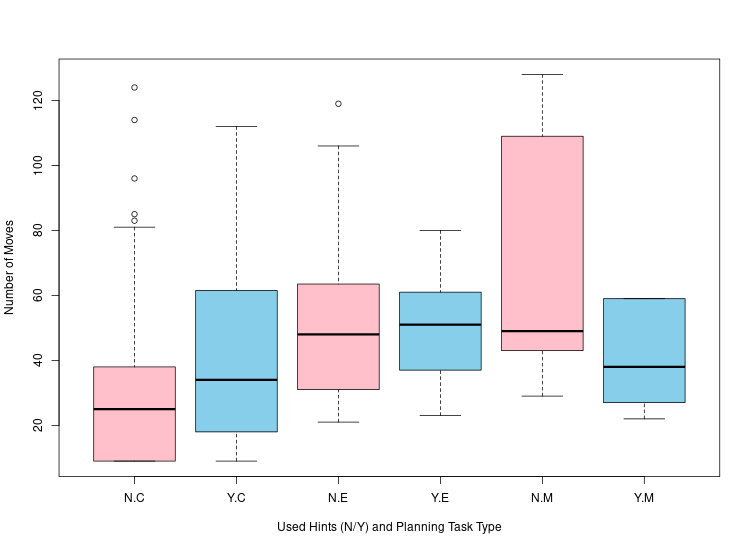
\includegraphics[width=0.8\columnwidth]{../img/lenbytype.png}
  \label{fig:lenbytype}
\end{figure}

\end{frame}

\begin{frame}{Moving the User's Solution Closer to the Optimal Solution - Metric 2}

\begin{itemize}
\item Solution length difference to the cost optimal solution between the condition (Y) and the control (N) groups \textbf{is not statistically significant}
\end{itemize}
\begin{figure}[tpb]
  \centering
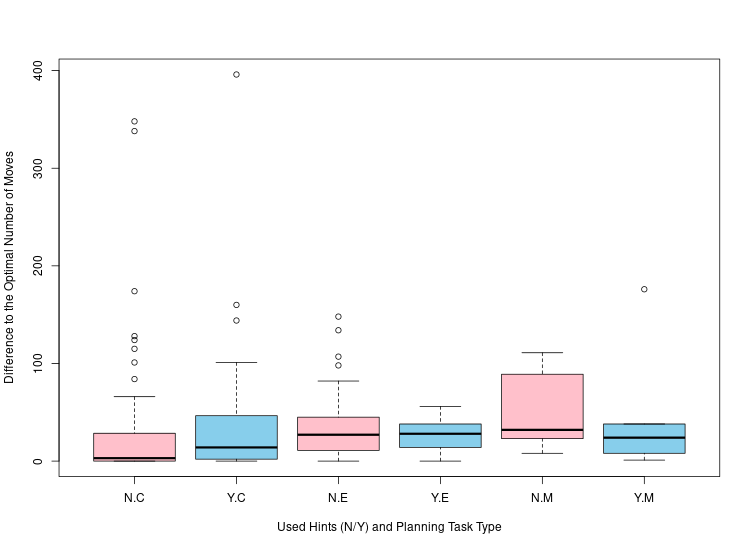
\includegraphics[width=0.7\columnwidth]{../img/lenoptbytype.png}
  \label{fig:lenoptbytype}
\end{figure}

\end{frame}

\begin{frame}{Moving the User's Solution Closer to the Optimal Solution - Metric 3}

\begin{itemize}
\item The latest times until the landmarks are achieved between the condition (Y) and the control (N) groups \textbf{is not statistically significant}
\end{itemize}
\begin{figure}[tpb]
  \centering
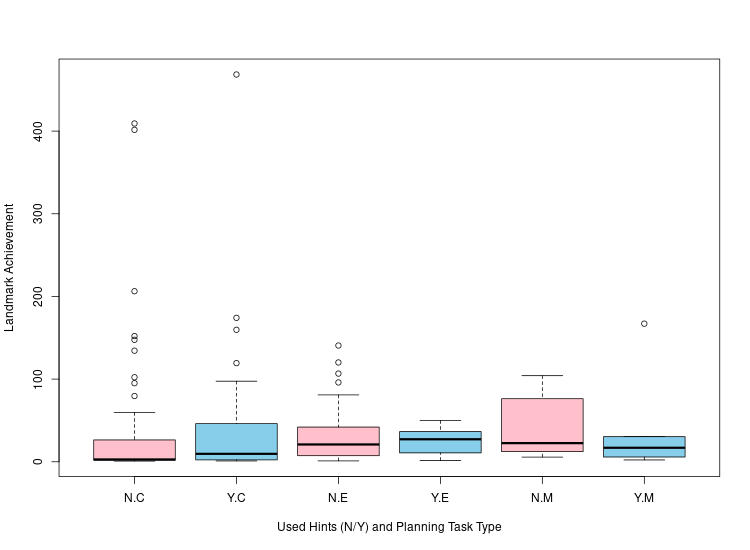
\includegraphics[width=0.7\columnwidth]{../img/achbytype.png}
  \label{fig:achbytype}
\end{figure}

\end{frame}

\begin{frame} {Moving the User's Solution Closer to the Optimal Solution - Metric 4}
\begin{itemize}
\item The number of times landmarks are lost and regained between the condition (Y) and the control (N) groups \textbf{is not statistically significant}
\end{itemize}
\begin{figure}[tpb]
  \centering
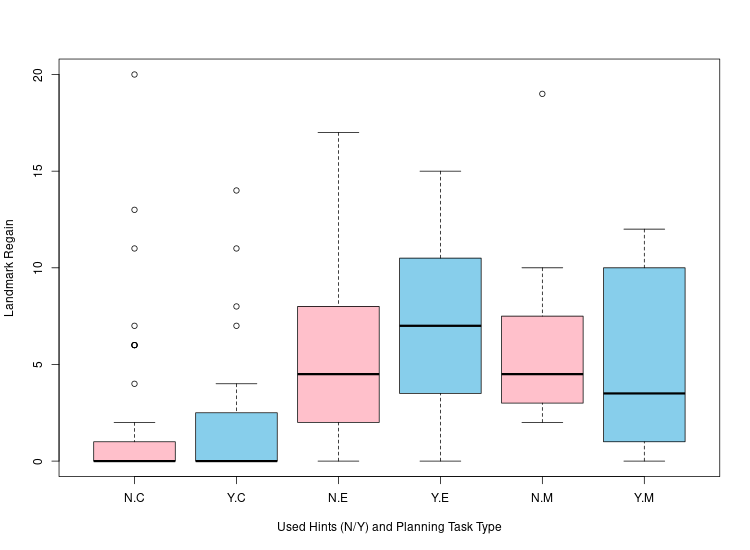
\includegraphics[width=0.7\columnwidth]{../img/regainbytype.png}
  \label{fig:regainbytype}
\end{figure}
\end{frame} %51, 52, 53, 54
\begin{frame}{Effect of Using Different Types of Help on Solution Length}
\begin{itemize}
\item Four help categories 
\begin{itemize}
\item participant watched the video and used the Interactive Human-aware Intervention (YY)
\item watched the help video but did not use the Interactive
Human-aware Intervention (YN)
\item participant did not watch the
help video but used the Interactive Human-aware Intervention (NY)
\item participant used neither type of help (NN)
\end{itemize}
\item Mean number of moves between different help types \textbf{is statistically significant}
\end{itemize}

\begin{table}
\begin{tabular}{|l|l|l|l|l|}
\hline
\multicolumn{1}{|c|}{\multirow{2}{*}{\begin{tabular}[c]{@{}c@{}}Planning Task\\ Type\end{tabular}}} & \multicolumn{4}{c|}{\begin{tabular}[c]{@{}c@{}}Number of Moves\\ median (mean)\end{tabular}} \\ \cline{2-5} 
\multicolumn{1}{|c|}{} & \multicolumn{1}{c|}{YY} & \multicolumn{1}{c|}{YN} & \multicolumn{1}{c|}{NY} & \multicolumn{1}{c|}{NN} \\ \hline
C & 78 (112) & 15 (27) & 54 (70) & 26 (25) \\ \cline{1-1}
E & 57 (62) & 33 (35) & 50 (56) & 34 (38) \\ \cline{1-1}
M & 41 (55) & 29 (32) & 32 (36) & 26 (28) \\ \hline
\end{tabular}
\end{table}

\end{frame} %55
\begin{frame}{Summary}
\begin{itemize}
\item Qualitatively human users prefer the ''\textbf{Show the next best move}'' hint
\item Quantitatively the use of Human-aware Intervention did not statistically significantly change the solution length, the difference to the optimal,  landmark achievement time and landmark regain
\item Use of different help types significantly affect the solution length
\item Need to strike a balance between revealing too much information   (i.e., complete solution) and too little information (i.e., next best move) about the planning problem.
\end{itemize}

\end{frame}

\begin{frame}{Concluding Remarks}
\begin{itemize}
\item \textbf{Contributions:}
\begin{itemize}
\item Intervention is viewed as two sub processes
\begin{itemize}
\item Intervention Recognition (proposed 3 solutions)
\item Intervention Recovery (proposed 1 solution)
\end{itemize}
\item Solutions combine automated planning and machine learning
\item Evaluated on synthetic domains and realistic data from human subject studies
\end{itemize}

\item \textbf{Future Work:}
\begin{itemize}
\item Explore different models of the actors' environment
\item Domain abstraction techniques to support intervention recovery
\item Ensuring longevity of interactive intervention models
\end{itemize}
\end{itemize}
\end{frame} %56,57

%\begin{frame}{Choice of Hint by Speed}
\begin{figure}[tpb]
  \centering
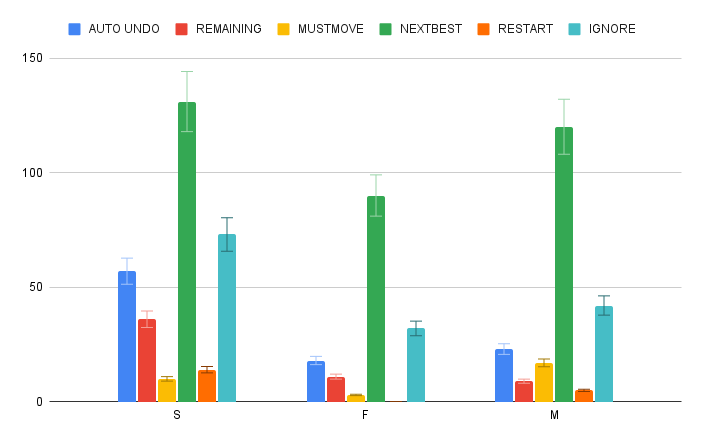
\includegraphics[width=0.8\columnwidth]{../img/speedreq.png}
  \caption{Number of requests for each hint type in slow (S), medium (M) and fast (F) solution groups.}
\end{figure}
\end{frame} %46
%\begin{frame}{Choice of Hint by Puzzle Type}
\begin{figure}[tpb]
  \centering
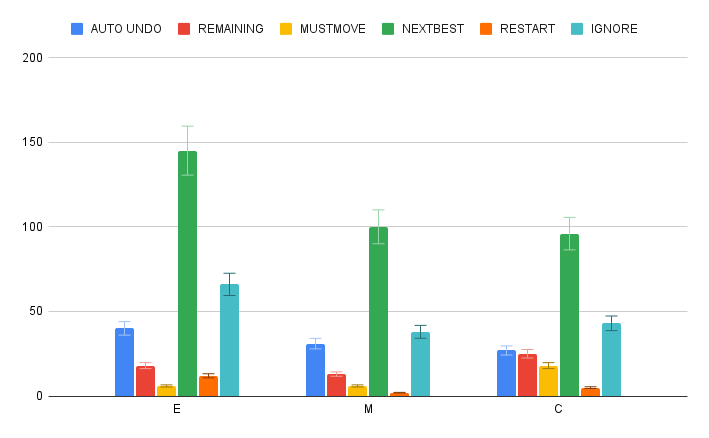
\includegraphics[width=0.8\columnwidth]{../img/typeandreq.png}
  \caption{Number of requests for each hint in the Rush Hour planning task types E, M, C with error bars.}
  \label{fig:groupandrequest}
\end{figure}

\end{frame} %47




\end{document}